\section{Messaging semantics}
In systems with asynchronous messaging, messaging semantics such as ordering guarantee, delivery guarantee cannot be provided by the message broker alone. The producers and consumers of messages must collaborate with the messages broker to achieve different levels of semantics. Therefore, in this section, before going into the evaluation, the general prerequisite for collaboration of the clients, which is true for all ESP platforms, is briefly recapped.
\subsection{General prerequisite}
\textbf{Strong ordering guarantee}\\
To achieve ordering guarantee of messages, the throughput must be compromised. On the message publishing side, at any time, messages from the same source must be published from only one producer instance. Otherwise, since concurrent producers publish events independently and are subject to different network conditions, the order of events cannot be preserved when they arrive at the ESP platform. Similarly for consumers, to guarantee that messages from the same source are processed in the correct order, concurrent consumption with multiple application instances is not permitted.

To have both concurrency and ordering guarantee, the concurrent instances must coordinate with each other to enforce the right order when publishing or consuming messages. Nevertheless, this method can introduce more overhead to the system.

Moreover, when a producer asynchronously send a message and proceed to the next one before receiving acknowledgement from the broker, if a message fails to reach the broker and is resent later, it is possible that another message may arrive in between causing their orders to be interchanged.
\begin{figure}[h]
	\centering
	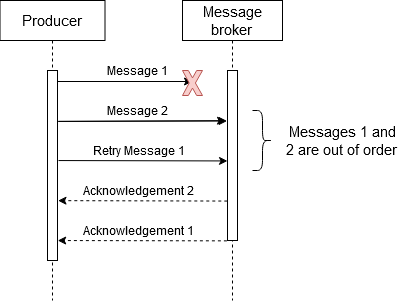
\includegraphics[width=6cm,height=4cm]{images/order.png}
	\caption{Asynchronous publishing and retrying causes out-of-order messages.}
	\label{fig:outorderretry}
\end{figure}

Therefore, in case the broker does not support detect out-of-order of asynchronously published messages, producer should only synchronously publish message one by one for ordering guarantee.


\textbf{At-most-once and At-least-once delivery semantics}\\
When a message is published, it can be lost along the way from producer to broker. Therefore, it is the responsibility of the producer to keep tracks of the sending status and resend messages if necessary. On the receiving side, after receiving and processing a message received from the broker, a consumer usually must perform two operations, namely, durably persisting the result of the processing and updating the current reading position on the source message stream to indicate that it has finished with the current message and will not receive it again. Since failures can non-deterministically occur between two operations, different order of these operations can result in different delivery guarantees. 

With at-most-once semantics, a producer can simply send messages in a fire-and-forget fashion without waiting for acknowledgements of successfully receiving from the message broker. Therefore, one of the key benefits of at-most-once guarantee is higher throughput since the producer is not impeded by the overhead introduced by acknowledging. When failures occur, messages may not reach the platform and are lost. When consuming a message, consumer must update its current reading position \underline{before} committing the calculated result from the message. In this way, if the consumer goes down before the result is persisted, it will continue with the next message upon restarting while the previous message will not be received again, and the corresponding result is simply lost.

For at-least-once semantics, messages producer must wait for acknowledgement from server for every message and is responsible for resending to avoid message loss. As a result, within one connection session, a message can appear on the message pipeline multiple times in case it is already received by the broker but the acknowledgement to the producer is lost. On the consumption side, for each received message, the consumer must mark it as being consumed and update the reading position only \underline{after} it has handled the message and durably persisted the result. In this way, if the consumer crashes after the result is stored but before the current reading position is updated, it will receive and process the message again after restarting and a new result will be generated along with the previously persisted result. In this case, duplication will be introduced between two connection sessions.
\begin{figure}[h]
	\centering
	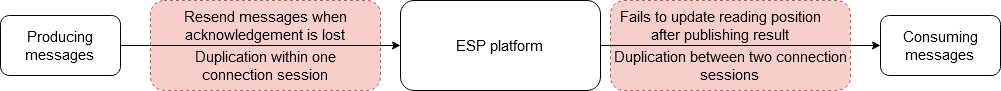
\includegraphics[width=\linewidth]{images/at-least-once-duplication.png}
	\caption{Duplication of messages with at-least-once delivery semantics.}
	\label{fig:messageduplication}
\end{figure}

\textbf{Exactly-once semantics}\\
Although it is physically not possible to ensure that each message is delivered and processed exactly once in a distributed system given the non-reliable nature of network \cite{exactlyoncenotpossible}, exactly-once processing semantics can still be realized on top of at-least-once guarantee. 

With at-least-once semantics, duplication can be introduced within one connection session or between two consecutive connection sessions. One possible solution is having the processing logic of the application to be idempotent so that multiple retries do not affect the end result. However, the feasibility of this approach depends on specific use cases.

Another approach is implementing deduplication mechanism on either the client or the message broker. The evaluation will focus on inspecting the support of this feature on the ESP platforms. 

\subsection{Evaluation}
\large \textbf{Apache Kafka}\\
\normalsize
\textbf{Strong ordering guarantee}\\
A Kafka topic comprises of one or more partitions. Kafka can guarantee that when two records are written to the same partition, they will be stored and delivered to consumers in the same order as their arriving order \cite{kafkaconfluentintro}.

On the consumer side, in a Kafka consumer group, each partition of the topic is assigned to only one consumer. There are no other competing consumers for each partition. As a result, the delivery model of Kafka guarantee that messages on a partition are delivered and processed in the right order.

On the producer side, all events from the same source must be sent to the same partition where order is guaranteed by Kafka. By default, records with the same key value will be published to the same partition. Therefore, producers must assign appropriate key value for each published message.

Asynchronous publishing of messages while ensuring order is also possible with Kafka. From Kafka 0.11, the idempotent producer is introduced \cite{kafkatransaction}. When this feature is enabled on a producer, for each targeted partition, each writing request will be assigned an incremental sequence number which will be used for deduplication on the broker in case of retrying. Thanks to this sequence number, Kafka can also tolerate up to 5 asynchronous publishing requests from one producer.

\textbf{At-most-once and At-least-once delivery semantics}\\
With Kafka producer, users have the flexibility to control the level of durability of published messages. Producer can be configured to wait for acknowledgements from only the leader partition, from all in-sync replicas or not wait for any confirmation from Kafka broker at all \cite{kafkaconfigurationproducer}. For the at-most-once guarantee, producer can be configured to send a record and immediately proceed to the next one without waiting for acknowledgement from the server. With the at-least-once guarantee, durability of published message must be ensured. Therefore, as elaborated in section \ref{section:eventstorage}, the producer must be configured to wait for the acknowledgements from all in-sync replicas to ensure that the published message is safely received and replicated by the Kafka server. Internally, if Kafka producer is configured to wait for acknowledgement from brokers, it will retry in case of failure until timeout. Therefore, there is no need to implement the retry logic in the application. 

On the Kafka consumer, by default, the offset number indicating the current reading position will be periodically persisted to Kafka. To have a better control over when to update the reading position, this should be disabled. The offset number should be manually committed before or after persisting the calculated result depending on the chosen delivery semantics.   

To sum up, Kafka supports both at-most-once and at-least-once delivery semantics with its clients.

\textbf{Exactly-once semantics}\\
From release 0.11 \cite{kafkatransaction}, Kafka provides mechanisms to protect against both types of duplication introduced by at-least-once semantics (figure \ref{fig:messageduplication}) and realize exactly-once semantics. 

To avoid duplicated messages by producer resending, the idempotent producer is introduced. Whenever a new producer instance is created and connected to Kafka, it is assigned a unique ID by the broker. When publishing messages to a partition, producer will add an incremental sequence number to every message along with its ID. By using these two values, the broker can uniquely identify a specific message sent by a producer on each partition and can discard any duplicated messages resulted from resending. 

To prevent duplication across two different connection sessions, Kafka provides the transaction feature. When a Kafka producer writes records to multiple partitions in a transaction, either all produced records are safely persisted or none of them is available to be read by other Kafka consumers. When Kafka consumer persists its current reading position to Kafka, internally this value is written to a special Kafka topic. Therefore, the act of updating reading position can be put in a transaction similarly to producing a normal record.

\begin{figure}[h]
	\centering
	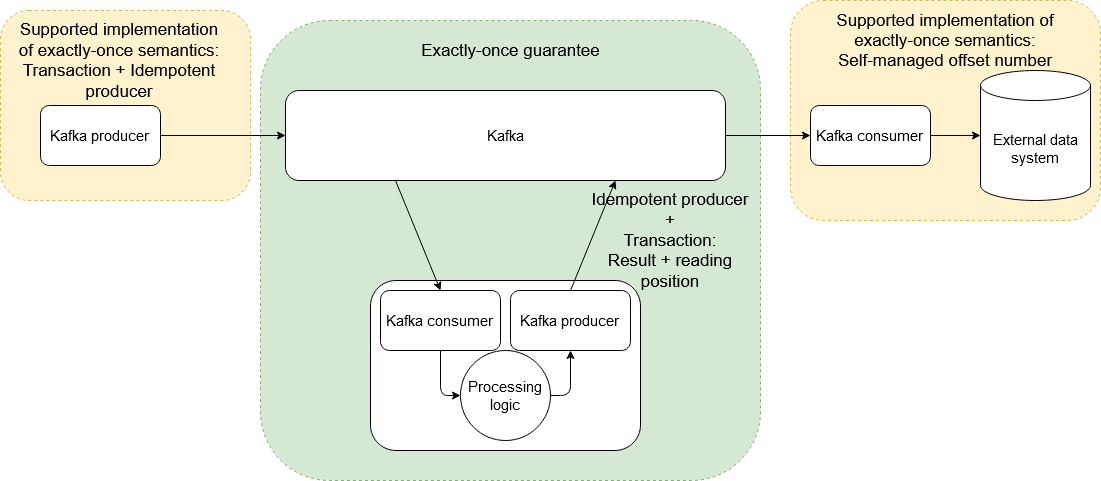
\includegraphics[width=\linewidth]{images/exactly-once-kafka.png}
	\caption{Support of exactly-once semantics on Kafka (\emph{green}: fully supported, \emph{yellow}: partly supported, \emph{red}: not supported).}
	\label{fig:exactlyoncekafka}
\end{figure}


For application which obtains data from Kafka topics with Kafka consumer and then produces new records back to Kafka, it can use Kafka producer to persist the result to output topics and commit the current reading position on input topics in a single transaction. In this way, even if the application crashes while producing records back to Kafka, when it restarts, it can start consuming records again from a clean state with the latest successfully committed result and reading position. Any result generated in the middle of a failed transaction will be discarded. 

In case of edge application which obtains data from an external system and produces records to Kafka, the application can produce records along with their related reading positions on the external system in a transaction. Upon restarting, application can retrieve the last committed position on Kafka and resume the processing on the external system accordingly. 

However, for edge consuming application which will write result to an external system, the transaction cannot span across its Kafka boundary. In this case, one possible approach is persisting atomically the reading position of the consumer along with the calculated result in the targeted external data system given that it supports transactions. Upon restarted, the consumer can retrieve the committed offset number and resume consumption accordingly. The delivery model of Kafka makes it easier to implement this since the reading position is only an offset number and can be controlled and persisted anywhere by the consumer.


\large \textbf{Apache Pulsar}\\
\normalsize
\textbf{Strong ordering guarantee}\\
A topic on Pulsar can either be non-partitioned or partitioned. Internally, a partition is also a normal non-partitioned topic. Pulsar guarantees that messages published to the same partition/non-partitioned topic will always be delivered to consumption side in the order in which they arrived at Pulsar \cite{pulsarconceptmessaging}.

If Pulsar consumer is used to consume messages, the Explicit and Failover subscription mode can be used to ensure the order of arriving messages. In the Explicit mode, there are no competing consumers for a topic regardless of being partitioned or not. With the Failover mode, similarly to Kafka consumer group, each partition will be assigned to only one consumer in the subscription while other consumers only take over when failures occur. Thus, each consumer in these two modes can receive all messages on a partition from Pulsar in the right order. If Pulsar reader is used, order of consumed messages is guaranteed since each reader can only be connected to a non-partitioned topic and grouping multiple readers for parallel reading of a topic is not possible. 

On producer side, if the topic is partitioned, appropriate key values must be assigned to every message to ensure that events from the same source will be produced to the same partition where order of delivery is guaranteed by Pulsar.

Regarding asynchronous publishing of messages, Pulsar also claims that a producer can have multiple asynchronous requests on the same connection to Pulsar while the order of messages received on the broker is still guaranteed \cite{pulsarinflight}.

\textbf{At-most-once and At-least-once delivery semantics}\\
When using Pulsar producer, it is not possible to publish messages in a fire-and-forget way. Internally, the producer always waits for confirmation from the broker and retries sending the messages if no acknowledgement is received until a specified timeout. As a result, a message can be duplicated on the stream. The Pulsar broker supports deduplication of resent messages. However, this will introduce overheads on both the producer for resending and the brokers for deduplication which does not comply with the key benefit of low overhead of at-most-once semantics. Therefore, in general, Pulsar producer does not support at-most-once. On the other hand, the Pulsar producer is very suitable for the at-least-once guarantee. Since the producer always waits for acknowledgement and retries sending message internally, no self-implementation of retry logic is needed.  

On the consuming side, the application must update the reading position (by either acknowledging if Pulsar consumer is used or persisting message ID of the consumed message if Pulsar reader is used) and durably persist the calculated in the appropriate order for the delivery semantics.

Considering both publishing and consuming sides, Pulsar clients only support at-least-once delivery semantics.

\textbf{Exactly-once semantics}\\
From release 1.20.0, Pulsar provides idempotent producer to discard any duplicated message introduced by producer retrying \cite{pulsaridemproducer}. With this feature, each producer must be assigned a globally unique name. Each message published to a Pulsar topic will be automatically assigned an incremental sequence ID by the producer. Pulsar broker will use the producer name and the sequence ID to uniquely identify each message published by a producer on a topic and discard any duplicated message resulted from retrying. 

For deduplication of duplicated messages created by consumer between two connection sessions, from release 2.7.0, Pulsar provides the transaction feature for Pulsar producer and consumer \cite{pulsartransaction}. With this new feature, users can publish messages to multiple Pulsar topics as well as acknowledge consumed message on numerous Pulsar source topics in one atomic operation. If the application fails during the transaction, all half-committed values will be discarded.  

For application which reads messages from Pulsar and produces results back to Pulsar, exactly-once semantics can be achieved. The transaction feature can be used to ensure that the application will always recover from a crash with a clean state on both source and output Pulsar topics.   

For application which processes data on external system and produces messages to Pulsar, it can use Pulsar producer to send messages and the corresponding reading positions on the external system to Pulsar in one transaction.  In this way, the application can resume the consumption on the external system after failure with the committed position on Pulsar to ensure the exactly-once semantics. 

In case of application which reads messages from Pulsar and writes result to an external system, the Pulsar transaction cannot span on both systems. In this case, exactly-once must be self-implemented. For instance, the Pulsar transaction can be integrated into the two-phase commit protocol \cite{twophasecommit} to acknowledge consumed messages on Pulsar and produce new messages to external system. This approach is used in the implementation of this connector to connect Apache Pulsar and Apache Flink \cite{pulsarflinkconnector}. However, this method depends on the availability of support for two-phase commit on destination system. Users can also use Pulsar reader to have more flexible control on the reading position on Pulsar. In this case, the message ID of the currently consume message on Pulsar can be persist together with the corresponding result to the external system to achieve atomicity similarly to Kafka.

The transaction feature is still in technical review phase. Therefore, this feature should not be used for production and exactly-once semantics is considered to be only partly supported on Apache Pulsar at the moment.


\begin{figure}[h]
	\centering
	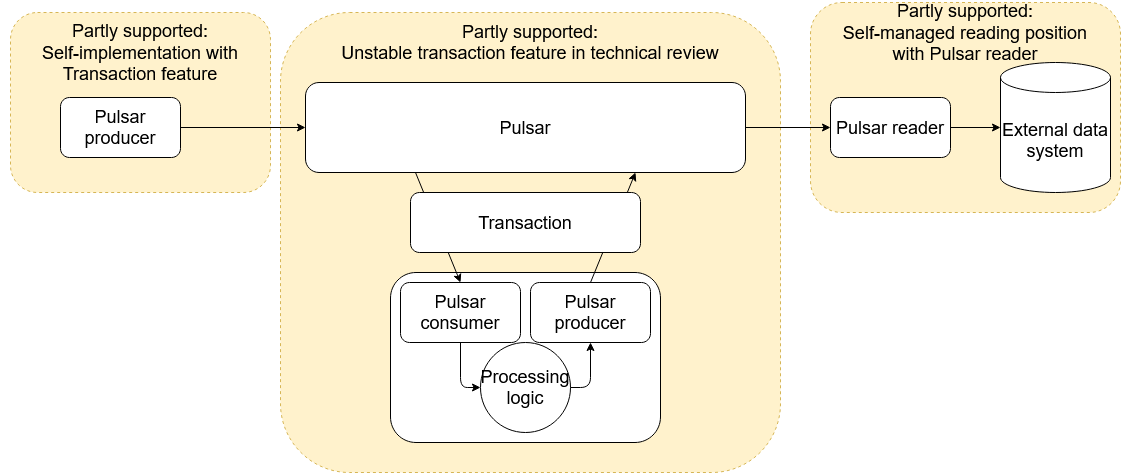
\includegraphics[width=\linewidth]{images/exactly-once-pulsar.png}
	\caption{Support of exactly-once semantics on Pulsar (\emph{green}: fully supported, \emph{yellow}: partly supported, \emph{red}: not supported).}
	\label{fig:exactlyoncepulsar}
\end{figure}




\large \textbf{NATS Streaming}\\
\normalsize
\textbf{Strong ordering guarantee}\\
Messages on NAT Streaming are organized into different channels. There is no lower level of partitioning of messages. NATS streaming can guarantee that when a subscriber consumes from a channel, messages are delivered in the same order as when they are published and persisted to the channel. This is not explicitly written in the document, but it is explained by NATS development team in discussions on GitHub \cite{natsorder}.

On the subscriber, to guarantee the order of messages, only normal subscription mode can be used. In this mode, each subscription has only one consumer without any other competing consumer \cite{natsconceptchannels}. Therefore, this single consumer can receive all messages on the channel in right order and process them sequentially.

Moreover, with its delivery model, NATS streaming actively pushes messages to subscriber and expects that these messages will be processed right away and acknowledged shortly after. Therefore, in case the consumption of a message takes longer time than the timeout for acknowledgement, the message can be resent out-of-order along with new messages. If the processing speed of client does not match the delivery of server, the sequence of delivered messages will not retain the right order anymore.
\begin{figure}[h]
	\centering
	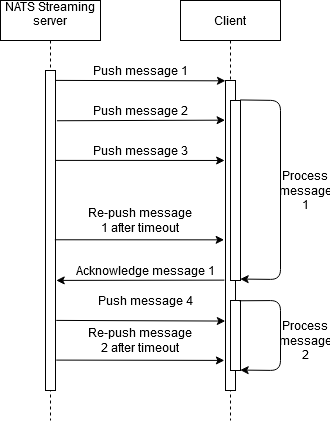
\includegraphics[width=5cm,height=7cm]{images/order-nats.png}
	\caption{NATS Streaming server redelivers messages out-of-order: message 1 and 2 are processed longer than the acknowledgement timeout and therefore are resent by server. Client sees the sequence of messages 1, 2, 3, 1, 4, 2.}
	\label{fig:ordernats}
\end{figure}

Therefore, the sending rate of the server must be limited to only one unacknowledged message at a time necessary to avoid out-of-order redelivery \cite{natsdevelopingacks}. As a result, it is not possible to receive messages in batch with NATS Streaming. 

On the producer side, messages must be published to the same channel where order is retained. Moreover, producer must synchronously send the messages one after another since the NATS server does not support protection against out-of-order caused by resending messages.  

\textbf{At-most-once and At-least-once delivery semantics}\\
Internally NATS producer always wait for acknowledgement from server after publishing a message. However, unlike Kafka and Pulsar, this producer does not retry internally to resend a message if it does not receive acknowledgement from the server. Thus, to have at-most-once guarantee on the publishing side, the publishing status returned by the producer can be simply ignored to realize fire-and-forget publishing. On the other hand, for at-least-once semantics, returned error from the producer should be handled with self-implemented retry logic to guarantee that the deliveries of all messages are successful.

NATS subscriber must acknowledge every consumed messages so that the server can continue to push next unacknowledged messages. However, the acknowledgement by NATS client to server is fire-and-forget \cite{natsorder}. The acknowledgment can be lost without the subscriber knowing about it which will cause the the message to be resent. If a consumer can perform deduplication to process each message exactly once, end-to-end at-most-once guarantee can still be realized. Nevertheless, as will be seen in the next evaluation section, end-to-end exactly-once guarantee cannot be achieved on NATS Streaming. As a result, at-most-once delivery guarantee is also not realizable by NATS Streaming.

On the other hand, at-least-once consumption of messages is possible with NATS clients. Consumer must update its reading position (by acknowledging the message with the server for durable subscription or checkpointing the reading position to external system for non-durable subscription) after it has durably published the calculated result. In case of non-durable subscription, the consumer still needs to send acknowledgement to the server. Nevertheless, when to acknowledge is irrelevant since the consumer only relies on the external checkpoint to resume the consumption. 

\textbf{Exactly-once semantics}\\
Currently, NATS Streaming server does not support detect and discard duplication within one connection session when a client resends a message multiple time. If deduplication is needed, it must be self-implemented on the application layer. 

For duplication introduced between connection sessions when client crashes before updating its current reading position, NATS Streaming also provides no deduplication mechanism. For an application which reads messages from NATS and publishes the results to another NATS channel, it is not possible to atomically publish new message and update reading position on source channel. Therefore, it is always possible that a message whose result is already published will be re-consumed and duplicated result will be generated. The same applies to application which publishes messages obtained from an external system to NATS Streaming.

For application which consumes messages from NATS and writes results to an external storage, it can use non-durable subscription and rely on the transactional feature of the sink system to store the sequence ID of consumed message and output value to achieve exactly-once. However, NATS Streaming server can always redeliver a message when it does not receive acknowledgement from client after timeout. There are also duplicated messages introduced to the channel from the upstream applications. Application must handle the deduplication of these messages as well.

As a result, in general, exactly-once semantics is not supported by NATS Streaming.


\begin{figure}[h]
	\centering
	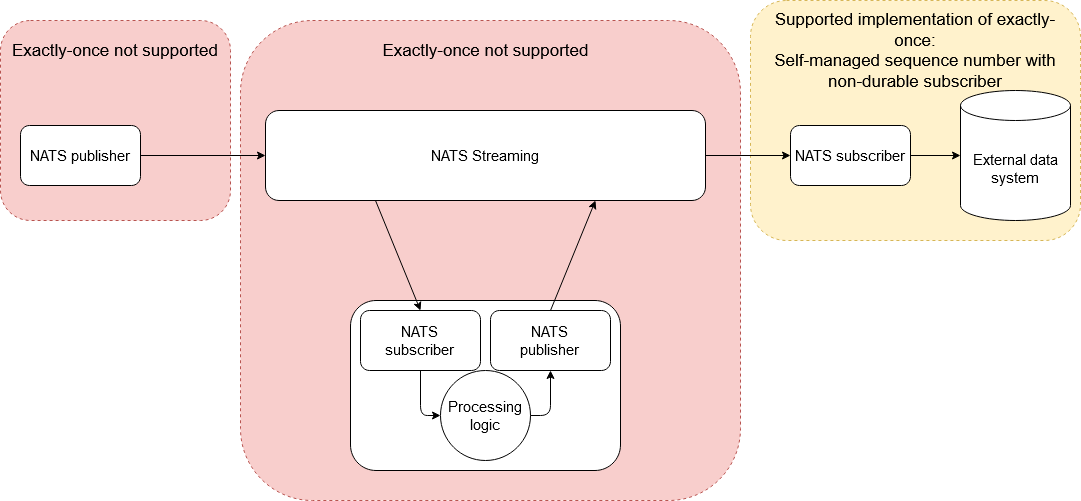
\includegraphics[width=\linewidth]{images/exactly-once-nats.png}
	\caption{Support of exactly-once semantics on NATS Streaming (\emph{green}: fully supported, \emph{yellow}: partly supported, \emph{red}: not supported).}
	\label{fig:exactlyoncenats}
\end{figure}






